%RL->MDP, Q, SARSA, SMDP, 
%MDP
%Model-based
%dynamic programming
%Dyna
%Model-free
%Q
%SARSA
\chapter{Background}
\label{ch:RL}

In this chapter, we introduce the basic concept of reinforcement learning (RL)
, the Markov decision process (MDP) and semi-Markov decision process (SMDP) formalisms. We describe the solution methods of MDPs, that include model-free and model-based 
methods. Then we review the concepts and algorithms in the hierarchical reinforcement learning (HRL) framework. 
We present a brief introduction of previous work in the RL field.
For more comprehensive introductions of MDP, SMDP and RL, please refer to the standard texts
\cite{Howard1960, Puterman94, SuttonIntro, KevinIntro}.
A more theoretic treatment of RL is provided by Bertsekas and Tsitsiklis \cite{Neurodynamic}.
Barto and Mahadevan provide an excellent review on HRL \cite{HRLSurvey}.

\section{Reinforcement learning}
\label{se:RL}
Reinforcement learning (RL) is a collection of methods which allow an agent to execute
a sequence of actions and improve its actions by a reinforcement mechanism.
In the RL setting, the environment can be modeled in several formalisms.
One of the most commonly adopted formalisms is Markov decision processes (MDPs).
An MDP assumes that the state of the environment is fully observable, and each action takes a single
step to finish. Semi-Markov decision processes (SMDPs) remove the latter assumption and allow
the action to take several time steps. Partially observable Markov decision processes (POMDPs) remove
the former assumption and the agent needs to decide the actions without access to the full state
of the environment.
MDPs and SMDPs are introduced in Sections \ref{se:MDP} and \ref{se:SMDP}.
POMDPs are orthogonal to our work, thus they will not be covered.

%Regardless of the underlying models of the environment, the objective of an RL method is
%to find an optimal policy for the model. 
%the MDP is unknown to the agent in the beginning. 
%The task of reinforcement learning
%consists of nding an optimal policy for the associated MDP. We will therefore
%refer to the underlying MDP as the model of the environment (or simply model
%if it is clear from the context which meaning of model is intended). The optimal
%policy is denoted by  and the corresponding utility function by V .

%TODO: why RL
%TODO: the challenge of RL

\section{Markov decision processes}
\label{se:MDP}
%In this work, we address the finite state Markov decision process (MDP) problem:

\begin{definition} A Markov decision process is formalized as a tuple $<S, A, P, R, I>$, where:
\begin{itemize}
    \item $S$ is a finite set of states of the environment.
    \item $A$ is a finite set of actions.
    \item $P:S \times A \times S \rightarrow [0, 1]$ is the transition function which defines a probability distribution over the possible next states.
    \item $R:S \times A \rightarrow \mathbb{R}$ is the reward function which defines the reward after executing a certain action at a certain state.
    \item $I:S \rightarrow [0, 1]$ specifies the initial state distribution.
 \end{itemize}
\end{definition}

Given a state of the environment, a policy $\pi: S \rightarrow A$ dictates what action should be performed at that state. 
The value function $V^{\pi}: S \rightarrow \mathbb{R}$ represents the expected cumulative reward when 
policy $\pi$ is followed from state $s$.

The value function is defined as:
\begin{align}
    V^{\pi}(s) &= E[R(s_0, \pi(s_0)) + \gamma R(s_1, \pi(s_1)) + \gamma^2 R(s_2, \pi(s_2)) + \dots | s_0 = s, \pi],
    \label{eq:defV}
\end{align}
where $\gamma \in [0, 1]$ is the discount factor which discounts the future reward to the present value.

The value function satisfies the Bellman equation \cite{Bellman57}:
\begin{equation}
    V^{\pi}(s) = \sum_{s'}P(s'|s, \pi(s))[R(s, \pi(s)) + \gamma V^{\pi}(s')]
    \label{eq:V}
\end{equation}

Similarly, the action-value function (or Q-function) represents the expected
cumulative reward after action $a$ is executed in state $s$ and policy $\pi$ is
followed thereafter.
The Q-function is defined as:
\begin{equation}
    Q^{\pi}(s, a) = E[\sum_{t=0}^{\infty}\gamma^t R(s_t, a_t) | s_0=s, a_0 = a, \pi]
\end{equation}

The Bellman equation for the Q-function is:
\begin{equation}
    Q^{\pi}(s, a) = \sum_{s'}P(s'|s, a)[R(s, a) + \gamma Q^{\pi}(s', \pi(s'))]
    \label{eq:Q}
\end{equation}

We are interesting in finding the optimal policy, which is the policy 
that achieves as high as the value of any other policies in all states.
It is defined as:
\begin{equation}
    \pi^*(s) = \argmax_{a \in A} [R(s, a) + \gamma \sum_{s'} P(s'|s, a)V^*(s')],
\end{equation}
where $V^*$ is the optimal value function. It satisfies the following equation:
\begin{equation}
    V^*(s) = \max_{\pi} V^{\pi} (s) = \max_{a \in A} [R(s, a) + \gamma \sum_{s'} P(s'|s, a)V^*(s')]
\end{equation}

Likewise, the optimal Q-function is the solution of the following equation:
\begin{equation}
    Q^*(s, a) = \max_{\pi} Q^{\pi}(s, a) = R(s, a) + \gamma \sum_{s'} P(s'|s, a) \max_{a' \in A} Q^*(s', a')
    \label{eq:optimalQ}
\end{equation}

%-------------------------------------------------------------------------
\section{Solution methods for MDPs}

There are several types of methods to solve an MDP problem. If the transition and reward functions are known as a priori, 
the optimal policy can be computed with dynamic programming (DP) algorithms.
%TODO: algorithms here? bellman equation
These methods are considered offline algorithms, since they are performed without
the interaction with the environment.

In the field of RL, people are more interested in solving the problems which
the underlying MDP is unknown in the beginning. 
Due to the lack of a priori model, it is necessary for the agent to interact with
the environment and collect samples to acquire the statistical knowledge of the MDP.
Therefore, the methods to solve these
problems are considered online algorithms.

%The lack of an apriori known model generates a need to sample the MDP to
%gather statistical knowledge about this unknown model. Depending on the kind
%of knowledge that is gathered, a distinction is made between model-based and
%model-free solution techniques.
Depend on how samples are processed, a distinction is made between model-based
and model-free methods. Model-based methods use samples to construct 
a model of environment and use the techniques such as dynamic programming
to compute the optimal policy from it.
On the other hand, model-free methods do not learn the model but directly learn
a policy or value function.
%A brief introduction of model-based and model-free methods are provided in
%Sections \ref{se:modelbased} and \ref{se:modelfree} respectively.

For both types of methods, a exploration policy is required to 
guide the sampling process.
The simplest strategy is to select an action which leads to the highest value. However, 
this strategy does not allow the agent to explore the states which are not visited before.
A better approach is to use $\epsilon$-greedy method. The method allows the agent to abandon the
best action and choose a random action with a very small probability $\epsilon$. The higher the probability, the more
likely that the agent would explore the new actions. However, if the exploration probability 
is too high, it will increase the time to converge.
%TODO: exploration vs exploitation


%according to the immediate reward and the estimated value of the next state


%There are 3 types of reinforcement learning algorithms -- dynamic programming (DP), Monte Carlo 
%methods, and temporal-difference (TD). Dynamic programming can compute the optimal policy, but it 
%requires a precise model of the environment. In most of the cases, the environment
%is too complex to be modeled precisely, and it is not easy to get the complete information about
%the environment. On the other hand, it is usually possible to use Monte Carlo method to sample the environment to
%get the partial information. 
%Like Monte Carlo method, TD uses sampling, therefore it does not require the 
%complete model of the environment. TD method is a bootstrapping method, similar to the dynamic 
%programming approach, it updates the new value function based on the previous one.

%Since a value function (or an action-value function) defines a policy in an MDP, one
%approach to find the optimal policy is to compute the optimal value (action-value) function
%first, and then extract the optimal policy from it. We call the algorithms utilizing this approach,
%value function algorithms. Another approach is to directly find the optimal policy.
%The methods using this approach are called policy search methods. In Sections 2.2.4.1 and
%2.2.4.2, we present a brief overview of the above two approaches to solve an MDP model.
%Value function (VF) methods attempt to find the optimal value (action-value) function
%and then extract an optimal policy from it. These algorithms have been extensively studied
%1998) and have yielded some remarkable empirical successes in a number of different domains,
%including learning to play checkers (Samuel, 1959), backgammon (Tesauro, 1994),
%job-shop scheduling (Zhang and Dietterich, 1995), dynamic channel allocation (Singh and
%Bertsekas, 1996), and elevator scheduling (Crites and Barto, 1998). We now briefly review
%some standard VF algorithms.
%If the model is known, then Equation 2.2 defines a system of equations, the solution to
%which yields the optimal value function. These equations may either be solved directly via
%solving a related linear program (e.g., Gordon (1999); de Farias (2002)), or by iteratively
%performing the update
%in the machine learning literature (Bertsekas and Tsitsiklis, 1996; Sutton and Barto,

%The lack of an apriori known model generates a need to sample the MDP to
%gather statistical knowledge about this unknown model. Depending on the kind
%of knowledge that is gathered, a distinction is made between model-based and
%model-free solution techniques.
%the agent needs to sample the MDP to acquire the knowledge about the MDP.
%The learning agent will take actions based on the current state. For the first step, the agent does not know anything about 
%the environment, therefore the agent has to choose the first action randomly. After the environment
%receives the action, it will provide a reward to the agent as a feedback. The reward can be either
%positive or negative. The agent adjusts the value function to maximize the expected reward in the future.

%The initial value of value function is 
%usually 0, but it is possible to set it to some high enough value to encourage exploration.
%It is important to evaluate the value function 
%correctly. If some actions with low expected reward are estimated as high, it degrades the
%performance of agent.
%In reinforcement learning, the environment can be modeled as an MDP but
%this MDP is unknown to the RL-agent. The task of reinforcement learning
%consists of nding an optimal policy for the associated MDP. We will therefore
%refer to the underlying MDP as the model of the environment (or simply model
%if it is clear from the context which meaning of model is intended). The optimal
%%In the RL setting, the environment is modeled as an MDP problem.

%However, the MDP is unknown to the RL agent. The objective of reinforcement learning is to 
%learn an optimal policy for the MDP. Since the MDP is unknown in the beginning, 
%the agent needs to sample the MDP to acquire the knowledge about the MDP.
%The learning agent will take actions based on the current state. For the first step, the agent does not know anything about 
%the environment, therefore the agent has to choose the first action randomly. After the environment
%receives the action, it will provide a reward to the agent as a feedback. The reward can be either
%positive or negative. The agent adjusts the value function to maximize the expected reward in the future.
%The initial value of value function is 
%usually 0, but it is possible to set it to some high enough value to encourage exploration.
%It is important to evaluate the value function 
%correctly. If some actions with low expected reward are estimated as high, it degrades the
%performance of agent.

%Other methods work without assuming prior knowledge of
%the model and operate by learning through experience in the environment; these are called
%online algorithms.
%Since a value function (or an action-value function) defines a policy in an MDP, one
%approach to find the optimal policy is to compute the optimal value (action-value) function
%first, and then extract the optimal policy from it. We call the algorithms utilizing this approach,
%value function algorithms. Another approach is to directly find the optimal policy.
%The methods using this approach are called policy search methods. In Sections 2.2.4.1 and
%2.2.4.2, we present a brief overview of the above two approaches to solve an MDP model.
%Value function (VF) methods attempt to find the optimal value (action-value) function
%and then extract an optimal policy from it. These algorithms have been extensively studied
%1998) and have yielded some remarkable empirical successes in a number of different domains,
%including learning to play checkers (Samuel, 1959), backgammon (Tesauro, 1994),
%job-shop scheduling (Zhang and Dietterich, 1995), dynamic channel allocation (Singh and
%Bertsekas, 1996), and elevator scheduling (Crites and Barto, 1998). We now briefly review
%some standard VF algorithms.
%If the model is known, then Equation 2.2 defines a system of equations, the solution to
%which yields the optimal value function. These equations may either be solved directly via
%solving a related linear program (e.g., Gordon (1999); de Farias (2002)), or by iteratively
%performing the update
%in the machine learning literature (Bertsekas and Tsitsiklis, 1996; Sutton and Barto,
%Other instances of offline VF algorithms are asynchronous value iteration and asynchronous
%policy iteration (Bertsekas and Tsitsiklis, 1996; Sutton and Barto, 1998).
%If the agent does not know the model of the domain, we may first try to interact with the
%environment to learn a model which is then used to compute optimal policies (e.g., Dyna
%(Sutton, 1991) and prioritized sweeping (Moore and Atkeson, 1993)). This is known as
%Model-based approach. Alternatively, we may try to learn the value (action-value) function
%directly and do not explicitly learn a model. This approach is referred to as model-free,
%in that the agent does not need to learn the transition probabilities. Most of the modelfree
%VF algorithms are instances of the temporal difference (TD) learning (Sutton, 1988),
%where the agent updates estimates of the value (action-value) function based in part on
%other estimates, without waiting for the true value. Two more popular TD methods are
%SARSA (Rummery and Niranjan, 1994) and Q-learning (Watkins, 1989).


%However, the MDP is unknown to the RL agent. The objective of reinforcement learning is to 
%learn an optimal policy for the MDP. Since the MDP is unknown in the beginning, 
%the agent needs to sample the MDP to acquire the knowledge about the MDP.
%The learning agent will take actions based on the current state. For the first step, the agent does not know anything about 
%the environment, therefore the agent has to choose the first action randomly. After the environment
%receives the action, it will provide a reward to the agent as a feedback. The reward can be either
%positive or negative. The agent adjusts the value function to maximize the expected reward in the future.
%The initial value of value function is 
%usually 0, but it is possible to set it to some high enough value to encourage exploration.
%It is important to evaluate the value function 
%correctly. If some actions with low expected reward are estimated as high, it degrades the
%performance of agent.


%Now that we have defined the MDP model, the next task is to solve it, i.e., to find an
%optimal policy and/or the optimal value function.5 There are variety of methods for achieving
%this. Some methods require knowing the transition probability and reward functions
%and are performed without access to an environment; these are considered offline algorithms.
%These are the standard dynamic programming (DP) algorithms from the field of
%operations research. Having the model allows the simulation of the domain so as to do
%planning to find the optimal value function and/or an optimal policy without interacting
%directly with the environment. Other methods work without assuming prior knowledge of
%the model and operate by learning through experience in the environment; these are called
%online algorithms.
%Since a value function (or an action-value function) defines a policy in an MDP, one
%approach to find the optimal policy is to compute the optimal value (action-value) function
%first, and then extract the optimal policy from it. We call the algorithms utilizing this approach,
%value function algorithms. Another approach is to directly find the optimal policy.
%The methods using this approach are called policy search methods. In Sections 2.2.4.1 and
%2.2.4.2, we present a brief overview of the above two approaches to solve an MDP model.
%Value function (VF) methods attempt to find the optimal value (action-value) function
%and then extract an optimal policy from it. These algorithms have been extensively studied
%1998) and have yielded some remarkable empirical successes in a number of different domains,
%including learning to play checkers (Samuel, 1959), backgammon (Tesauro, 1994),
%job-shop scheduling (Zhang and Dietterich, 1995), dynamic channel allocation (Singh and
%Bertsekas, 1996), and elevator scheduling (Crites and Barto, 1998). We now briefly review
%some standard VF algorithms.
%If the model is known, then Equation 2.2 defines a system of equations, the solution to
%which yields the optimal value function. These equations may either be solved directly via
%solving a related linear program (e.g., Gordon (1999); de Farias (2002)), or by iteratively
%performing the update
%in the machine learning literature (Bertsekas and Tsitsiklis, 1996; Sutton and Barto,
%Other instances of offline VF algorithms are asynchronous value iteration and asynchronous
%policy iteration (Bertsekas and Tsitsiklis, 1996; Sutton and Barto, 1998).
%If the agent does not know the model of the domain, we may first try to interact with the
%environment to learn a model which is then used to compute optimal policies (e.g., Dyna
%(Sutton, 1991) and prioritized sweeping (Moore and Atkeson, 1993)). This is known as
%Model-based approach. Alternatively, we may try to learn the value (action-value) function
%directly and do not explicitly learn a model. This approach is referred to as model-free,
%in that the agent does not need to learn the transition probabilities. Most of the modelfree
%VF algorithms are instances of the temporal difference (TD) learning (Sutton, 1988),
%where the agent updates estimates of the value (action-value) function based in part on
%other estimates, without waiting for the true value. Two more popular TD methods are
%SARSA (Rummery and Niranjan, 1994) and Q-learning (Watkins, 1989).


\subsection{Model-free methods}
\label{se:modelfree}
Most of the model-free methods fall into the category of the temporal difference (TD)
learning. The main idea of temporal difference learning methods is to iteratively
estimate the new values based on the old estimates. After the agent selects an action,
the value of the previous state is updated based on the immediate reward and the 
value of current state.

The equation to update the value function in TD learning is:
\begin{displaymath}
   V(S_t) \leftarrow V(S_t) + \alpha [r_{t+1} + \gamma V(S_{t+1}) - V(S_t)],
\end{displaymath}
where $V(s_t)$ is the value function of the state $s_t$. $V(s_t)$ is the expected reward when
the agent reaches state $s_t$. $r_{t+1}$ is the reward given to the agent when it chooses
the action at state $s_t$.

SARSA\cite{Rummery94} and Q-learning\cite{Watkins89} are the most popular TD
methods. SARSA is an on-policy TD approach, which indicates that it learns
from the current policy. Different from other TD approaches, SARSA updates the
Q-value from the value of the next state-action pair. The Q-value is
updated by:

\begin{displaymath}
    Q(s_t, a_t) \leftarrow Q(s_t, a_t) + \alpha [r_{t+1} + \gamma Q(s_{t+1}, a_{t+1})-Q(s_t, a_t)],
\end{displaymath}
where $Q(s, a)$ is the expected reward when the agent takes the action $a$ at
the state $s$. $\alpha$ is a constant step-size parameter. $\gamma$ is the
discount factor.

\begin{center}
\begin{tabular}{@{}lp{6cm}@{}}
\hline
Algorithm: SARSA\\
\hline
Initialize $Q(s, a)$ arbitrarily\\
Repeat (for each episode):\\
\ \ \ \ \ \ Initialize $s$\\
\ \ \ \ \ \ Choose $a$ based on $s$ using policy derived from $Q$ (e.g., $\epsilon$-greedy method)\\
\ \ \ \ \ \ Repeat (for each step of episode):\\
\ \ \ \ \ \ \ \ \ \ \ \ Take action $a$, obtain reward $r$ and next state $s'$ from the environment\\
\ \ \ \ \ \ \ \ \ \ \ \ Choose $a'$ based on $s'$ using policy derived from $Q$ (e.g., $\epsilon$-greedy method)\\
\ \ \ \ \ \ \ \ \ \ \ \ $Q(s, a) \leftarrow Q(s, a) + \alpha [r + \gamma Q(s', a')-Q(s, a)]$\\
\ \ \ \ \ \ \ \ \ \ \ \ $s \leftarrow s'$\\
\ \ \ \ \ \ \ \ \ \ \ \ $a \leftarrow a'$\\
\ \ \ \ \ \ Until $s$ is terminal\\
\hline  
\end{tabular}
\end{center}


%\section{Q-Learning}
%\label{se:Q-Learning}
Q-Learning is an off-policy TD approach. Compared to SARSA, Q-Learning updates
the Q value by the highest value of the next possible state-action, rather than the 
next state-action executed by the agent.  
The Q value is updated by:
\begin{displaymath}
   Q(s_t, a_t) \leftarrow Q(s_t, a_t) + \alpha [r_{t+1}+\gamma \max_a Q(s_{t+1},a)-Q(s_t,a_t)],
\end{displaymath}
where $\max_a Q(s_{t+1},a)$ is the highest value of the next possible state-action. 

\begin{center}
\begin{tabular}{@{}lp{6cm}@{}}
\hline
Algorithm: Q-Learning\\
\hline
Initialize $Q(s, a)$ arbitrarily\\
Repeat (for each episode):\\
\ \ \ \ \ \ Initialize $s$\\
\ \ \ \ \ \ Repeat (for each step of episode):\\
\ \ \ \ \ \ \ \ \ \ \ \ Choose $a$ based on $s$ using policy derived from $Q$ (e.g., $\epsilon$-greedy method)\\
\ \ \ \ \ \ \ \ \ \ \ \ Take action $a$, obtain reward $r$ and next state $s'$ from the environment\\
\ \ \ \ \ \ \ \ \ \ \ \ $Q(s, a) \leftarrow Q(s, a) + \alpha [r + \gamma max_{a'} Q(s', a')-Q(s, a)]$\\
\ \ \ \ \ \ \ \ \ \ \ \ $s \leftarrow s'$\\
\ \ \ \ \ \ Until $s$ is terminal\\
\hline  
\end{tabular}
\end{center}

\subsection{Model-based methods}
\label{se:modelbased}
Unlike model-free methods which adopt the trial-and-error learning process,
model-based methods construct a model of the environment from the samples and
conduct a planning process over it. With the constructed model, these methods
can predict the outcome of the agent's action, and choose an optimal action
that can achieve the highest predictive reward. Since this type of methods
makes efficient use of samples, they often require fewer samples to learn a
good policy than model-free methods. They are important to the applications
where computation is cheap and the interactions of the environment are
expensive.

A straightforward approach is to build the model by learning the transition function and
reward function, then use dynamic programming (DP) to compute the solution of
Bellman equation (Equation \ref{eq:optimalQ}).

The solution of Bellman equation is unique, but there might be several policies
which can have the same value function. The most well-known dynamic
programming algorithms are value iteration \cite{Bellman57} and policy
iteration \cite{Howard1960}.

Value iteration iteratively apply the Bellman equation to update the
values for all possible states. The value function will converge
usually in few iterations. 

\begin{center}
\begin{tabular}{@{}lp{6cm}@{}}
\hline
Algorithm: Value Iteration\\
\hline
Initialize $V(s)$ arbitrarily\\
Repeat:\\
\ \ \ for $s \in S$ do\\
\ \ \ \ \ \ $V(s) \leftarrow \max_a [R(s, a) + \gamma \sum_{s'} P(s'|s, a)]V(s')$\ \ \ \ \ \ \ \ \ \ \ \ \ \ \ \ \ \ \ \ \ \ \ \ \ \ \ \ \ \ \ \ \ \ \ \ \ \ \ \ \ \ \ \ \ \ \ \ \ \ \ \ \ \ \ \ \ \ \\
\ \ \ end for\\
Until maximal update smaller than $\delta$\\
\hline  
\end{tabular}
\end{center}

The policy iteration algorithm separates the iterative process into two stages. The first stage is policy evaluation, which computes the value function for
current policy. The second stage is policy improvement, which improve the
policy by choosing a better action based on the value function computed in
previous stage.

\begin{center}
\begin{tabular}{@{}lp{6cm}@{}}
\hline
Algorithm: Policy Iteration\\
\hline
Initialize $\pi_1$ arbitrarily\\
$k \leftarrow 1$\\
Repeat:\\
\ \ \ Repeat:\\
\ \ \ \ \ \ for $s \in S$ do\\
\ \ \ \ \ \ \ \ \ $Q^{\pi_k}(s, a) \leftarrow [R(s, \pi_k(s)) + \gamma \sum_{s'} P(s'|s, \pi_k(s)) Q^{\pi_k}(s', \pi_k(s))]$\ \ \ \ \ \ \ \ \ \ \ \ \ \ \ \ \ \ \ \ \ \ \ \ \ \ \ \ \ \ \ \ \ \ \ \ \ \ \ \ \ \ \ \ \ \ \ \ \\
\ \ \ \ \ \ end for\\
\ \ \ Until maximal update smaller than $\delta$\\
\ \ \ for $s \in S$ do\\
\ \ \ \ \ \ $\pi_{k+1}(s) \leftarrow \argmax_a Q^{\pi_k}(s', a)$\\
\ \ \ end for\\
\ \ \ $k \leftarrow k + 1$\\
Until $\pi_{k+1} = \pi_{k}$\\
\hline  
\end{tabular}
\end{center}

Another popular class of model-based methods is the Dyna architecture \cite{Dyna}.
Dyna \cite{Dyna} is to use the learned model to generate extra experiences through
the simulating process, but the underlying learning algorithm is still a TD method.
%The idea of the Dyna architecture is to use a model-free solution technique
%(such as the ones that will be described in the next section), but at the same
%time learn a model of the environment as in the certainty equivalent method.
%This model can then be used to generate extra experience through simulation.
%There are some other methods that build on this idea. Prioritized sweeping
%[Moore and Atkeson, 1993] for instance does not use a uniform distribution
%when generating extra experience but prioritizes them based on their change
%in values.
%2.2.2 Mo

%Although the term model-based reinforcement learning is sometimes used to
%refer to solution methods for problems where the MDP is known, we use modelbased
%RL in the traditional sense where methods are considered that do not
%know the model of the world a priori but that do operate by learning this
%model2. This category of approaches is especially important for applications
%where computation is considered to be cheap and real-world experience costly.
%equivalent method. The idea is to learn the transition and reward function
%by exploring the environment and keeping statistics about the results of each
%action. Once these functions are learned, a dynamic programming approach can
%be used to compute an optimal policy. Dynamic programming (DP) refers to
%a class of algorithms that are able to compute optimal policies given a perfect
%model of the environment as an MDP. Since this dissertation only deals with
%the reinforcement learning setting of the sequential decision making problem,
%Central in dynamic programming techniques is the so-called Bellman Equation
%[Bellman, 1965] or dynamic programming equation. This equation arises
%from rewriting the denition of the value function. Assuming the discounted
%cumulative future reward as optimality criterium (Equation 2.1), the following
%Bellman Equation is obtained:
%X
%s02S
%T(s; (s); s0)V (s0) (2.2)
%The solution for this set of equations (there is one equation for every state)
%gives the optimal value function V . Note that this solution is unique, but there
%can be several dierent policies that have the same value function. Usually
%an iterative algorithm is used to compute a solution. The two basic methods
%are value iteration [Bellman, 1957] and policy iteration [Howard, 1960]. Value
%iteration (shown in Algorithm 2.1) uses the Bellman equation to iteratively
%compute the optimal value function. The policy iteration algorithm (shown in
%Algorithm 2.2) interleaves a policy evaluation step, which computes the value
%function for the current policy using Equation 2.2, and a policy improvement
%step which changes the policy by choosing a better action in a certain state
%based on the policy evaluation.



%\section{}
%SARSA is a on-policy TD approach. On-policy indicates that it learns from the current policy.
%Different from other TD approaches, SARSA updates the Q value of the current state-action from the next state-action.
%The Q value is updated by:
%\begin{displaymath}
    %Q(s_t, a_t) \leftarrow Q(s_t, a_t) + \alpha [r_{t+1} + \gamma Q(s_{t+1}, a_{t+1})-Q(s_t, a_t)],
%\end{displaymath}
%where $Q(s, a)$ is the value function for state-pair, and it is the expected reward when the agent takes
%the action $a$ at the state $s$. $\alpha$ is step-wise, which controls the learning rate. 
%$\gamma$ is the discount factor.

%\begin{center}
%\begin{tabular}{@{}lp{6cm}@{}}
%\hline
%Algorithm: Dyna-Q\\
%\hline
%Initialize $Q(s, a)$ and $Model(s, a)$\\
%Repeat (for each episode):\\
%\ \ \ \ Repeat (for each step of episode):\\
%\ \ \ \ \ \ \ \ $s \leftarrow$ the current state\\
%\ \ \ \ \ \ \ \ Choose $a$ based on $s$ using policy derived from $Q$ (e.g., $\epsilon$-greedy method)\\
%\ \ \ \ \ \ \ \ Take action $a$, obtain reward $r$ and next state $s'$ from the environment\\
%\ \ \ \ \ \ \ \ $Q(s, a) \leftarrow Q(s, a) + \alpha [r + \gamma max_{a'} Q(s', a')-Q(s, a)]$\\
%\ \ \ \ \ \ \ \ $Model(s, a) \leftarrow s', r$
%\ \ \ \ \ \ \ \ Repeat $N$ times:
%\ \ \ \ \ \ \ \ \ \ \ \ $s \leftarrow $ random previously observed state
%\ \ \ \ \ \ \ \ \ \ \ \ $a \leftarrow $ random action previously taken in $s$
%\ \ \ \ \ \ \ \ \ \ \ \ $s', r \leftarrow Model(s, a)$ 
%\ \ \ \ \ \ \ \ \ \ \ \ $Q(s, a) \leftarrow Q(s, a) + \alpha [r + \gamma max_{a'} Q(s', a')-Q(s, a)]$\\
%\hline  
%\end{tabular}
%\end{center}

%\section{The Dyna Architecture}
%SARSA is a on-policy TD approach. On-policy indicates that it learns from the current policy.
%Different from other TD approaches, SARSA updates the Q value of the current state-action from the next state-action.
%The Q value is updated by:
%\begin{displaymath}
    %Q(s_t, a_t) \leftarrow Q(s_t, a_t) + \alpha [r_{t+1} + \gamma Q(s_{t+1}, a_{t+1})-Q(s_t, a_t)],
%\end{displaymath}
%where $Q(s, a)$ is the value function for state-pair, and it is the expected reward when the agent takes
%the action $a$ at the state $s$. $\alpha$ is step-wise, which controls the learning rate. 
%$\gamma$ is the discount factor.

%\begin{center}
%\begin{tabular}{@{}lp{6cm}@{}}
%\hline
%Algorithm: Dyna-Q\\
%\hline
%Initialize $Q(s, a)$ and $Model(s, a)$\\
%Repeat (for each episode):\\
%\ \ \ \ Repeat (for each step of episode):\\
%\ \ \ \ \ \ \ \ $s \leftarrow$ the current state\\
%\ \ \ \ \ \ \ \ Choose $a$ based on $s$ using policy derived from $Q$ (e.g., $\epsilon$-greedy method)\\
%\ \ \ \ \ \ \ \ Take action $a$, obtain reward $r$ and next state $s'$ from the environment\\
%\ \ \ \ \ \ \ \ $Q(s, a) \leftarrow Q(s, a) + \alpha [r + \gamma max_{a'} Q(s', a')-Q(s, a)]$\\
%\ \ \ \ \ \ \ \ $Model(s, a) \leftarrow s', r$
%\ \ \ \ \ \ \ \ Repeat $N$ times:
%\ \ \ \ \ \ \ \ \ \ \ \ $s \leftarrow $ random previously observed state
%\ \ \ \ \ \ \ \ \ \ \ \ $a \leftarrow $ random action previously taken in $s$
%\ \ \ \ \ \ \ \ \ \ \ \ $s', r \leftarrow Model(s, a)$ 
%\ \ \ \ \ \ \ \ \ \ \ \ $Q(s, a) \leftarrow Q(s, a) + \alpha [r + \gamma max_{a'} Q(s', a')-Q(s, a)]$\\
%\hline  
%\end{tabular}
%\end{center}

%--------------------------------

%The lack of an apriori known model generates a need to sample the MDP to
%gather statistical knowledge about this unknown model. Depending on the kind
%of knowledge that is gathered, a distinction is made between model-based and
%model-free solution techniques.
%2.2.1 Model-Based Solution Techniques
%Although the term model-based reinforcement learning is sometimes used to
%refer to solution methods for problems where the MDP is known, we use modelbased
%RL in the traditional sense where methods are considered that do not
%know the model of the world a priori but that do operate by learning this
%model2. This category of approaches is especially important for applications
%where computation is considered to be cheap and real-world experience costly.
%2Another term for these kind of algorithms is indirect reinforcement learning.
%2.2. SOLUTION METHODS 17
%2.2.1.1 Certainty Equivalent Method
%One straightforward method that falls within this category is the certainty
%equivalent method. The idea is to learn the transition and reward function
%by exploring the environment and keeping statistics about the results of each
%action. Once these functions are learned, a dynamic programming approach can
%be used to compute an optimal policy. Dynamic programming (DP) refers to
%a class of algorithms that are able to compute optimal policies given a perfect
%model of the environment as an MDP. Since this dissertation only deals with
%the reinforcement learning setting of the sequential decision making problem,
%dynamic programming techniques are only briey discussed.
%Central in dynamic programming techniques is the so-called Bellman Equation
%[Bellman, 1965] or dynamic programming equation. This equation arises
%from rewriting the denition of the value function. Assuming the discounted
%cumulative future reward as optimality criterium (Equation 2.1), the following
%Bellman Equation is obtained:
%The solution for this set of equations (there is one equation for every state)
%gives the optimal value function V . Note that this solution is unique, but there
%can be several dierent policies that have the same value function. Usually
%an iterative algorithm is used to compute a solution. The two basic methods
%are value iteration [Bellman, 1957] and policy iteration [Howard, 1960]. Value
%iteration (shown in Algorithm 2.1) uses the Bellman equation to iteratively
%compute the optimal value function. The policy iteration algorithm (shown in
%Algorithm 2.2) interleaves a policy evaluation step, which computes the value
%function for the current policy using Equation 2.2, and a policy improvement
%step which changes the policy by choosing a better action in a certain state
%based on the policy evaluation.
%Algorithm 2.1 Value Iteration
%1:    some small value
%2: V1   initial value function
%3: k   1
%4: repeat
%5: for s 2 S do
%6: Vk+1(s)   maxa
%
%R(s; a) + 

%P
%
%7: end for
%8: k   k + 1
%9: until maximal update smaller than 
%18 CHAPTER 2. REINFORCEMENT LEARNING
%Algorithm 2.2 Policy Iteration
%1: 1   initial policy
%2: k   1
%3: repeat
%4: //Compute the value function of policy k by solving the equations
%5: V k (s) := R(s; k(s)) + 

%P
%6: for s 2 S do
%7: // Policy improvement step
%8: k+1(s)   argmaxa2A
%P
%9: k   k + 1
%10: end for
%The most important drawback of the certainty equivalent method is the
%crisp devision between the learning phase and the acting phase: the agent will
%only start to show intelligent behavior once he has learned a full and perfect
%model. It has furthermore been shown that random exploration might not be
%very ecient to gather information that can build the full model [Koenig and
%Simmons, 1993].
%2.2.1.2 The Dyna Architecture
%A more ecient model-based approach is the Dyna architecture [Sutton, 1991].
%The idea of the Dyna architecture is to use a model-free solution technique
%(such as the ones that will be described in the next section), but at the same
%time learn a model of the environment as in the certainty equivalent method.
%This model can then be used to generate extra experience through simulation.
%There are some other methods that build on this idea. Prioritized sweeping
%[Moore and Atkeson, 1993] for instance does not use a uniform distribution
%when generating extra experience but prioritizes them based on their change
%in values.


\section{Semi-Markov decision processes}
\label{se:SMDP}

Semi-Markov decision processes (SMDPs) \cite{Puterman94} extend MDPs to handle
the actions which may take several steps to finish. It allows us to handle the
problem which the agent cannot make a decision for every step. The state may
be updated several times between each decision made by the agent. SMDPs
provide a way to model these temporal-extended actions, which make them an
important tool to describe the environment of hierarchical reinforcement
learning.

\begin{definition} A semi-Markov decision process (SMDP) is formalized as a tuple $<S, A, P, R>$, where:
\begin{itemize}
    \item $S$ is a finite set of states of the environment.
    \item $A$ is a finite set of actions.
    \item $P:S \times \mathbb{N} \times A \times S \rightarrow [0, 1]$ is a
        multi-step transition function. $P(s', N | s, a)$ denotes the
        probability that state is transited from  $s$ to $s'$ after action $a$
        is taken at state $s$ and finished in exact $N$ steps.
    \item $R:S \times \mathbb{N} \times A \rightarrow \mathbb{R}$ is the reward function which defines the reward after executing a certain action at a certain state.
    \item $I:S \rightarrow [0, 1]$ specifies the initial state distribution.
 \end{itemize}
\end{definition}

The formalism of SMDP is similar to an MDP, except that the transition function and reward function
now include the duration of actions. 

The definition of value function for SMDP is:
\begin{equation}
    V^{\pi}(s) = E[R(s_0, \pi(s_0)) + \gamma^{N_0} R(s_1, \pi(s_1)) + \gamma^{N_1} R(s_2, \pi(s_2)) + \dots | s_0 = s, \pi]
\end{equation}
The definition is similar to equation \ref{eq:defV}, except that the reward is discounted by
the duration of actions.

The Bellman equation for SMDP can be described as:
\begin{equation}
    V^{\pi}(s) = \sum_{s', N}P(s', N|s, \pi(s))[R(s', N|s, \pi(s)) + \gamma^N V^{\pi}(s')],
    \label{eq:SMDPV}
\end{equation}

Similarly, the Q-function for SMDP is defined as:
\begin{equation}
    Q^{\pi}(s, a) = \sum_{s', N}P(s', N|s, a)[R(s', N|s, a) + \gamma^N Q^{\pi}(s', \pi(s'))].
    \label{eq:SMDPQ}
\end{equation}

The optimal value function and Q-function satisfy the following equations:
\begin{equation}
    V^*(s) = \max_{a \in A} [R(s, a) + \sum_{s', N} \gamma^N P(s', N|s, a)V^*(s')]
\end{equation}
\begin{equation}
    Q^*(s, a) = R(s, a) + \sum_{s', N} \gamma^N P(s', N|s, a) \max_{a' \in A} Q^*(s', a')
\end{equation}

%The Bellman equation for SMDP can be described as:
%\begin{equation}
    %V*(s) = \sum_{s', N}P(s', N|s, \pi(s))[R(s', N|s, \pi(s)) + \gamma^N V^{\pi}(s')],
%\end{equation}

%Similarly, the Q-function is defined as:
%\begin{equation}
    %Q^{\pi}(s, a) = \sum_{s', N}P(s', N|s, a)[R(s', N|s, a) + \gamma^N Q^{\pi}(s', \pi(s'))].
    %\label{eq:Q}
%\end{equation}

%\begin{equation}
    %Q^{\pi}(s, a) = \sum_{s', N}P(s', N|s, a)[R(s', N|s, a) + \gamma^N Q^{\pi}(s', \pi(s'))].
    %\label{eq:SMDPQ}
%\end{equation}
%Now lets us extends action set $A$ to include composite actions.

%The transition function $P$ and $R$ are modified to include the time to accomplish each composite action:
%\begin{equation}
    %R(s, a) = \sum^{\infty}_{k=0} \gamma^k r_k
%\end{equation}

%The value function needs to be modified as:
%\begin{equation}
    %V^{\pi}(s) = \sum_{s'}P(s'|s, \pi(s))[R(s, \pi(s), t) + \gamma^N V^{\pi}(s')],
%\end{equation}
%where $N$ is the number of steps for the action $\pi(s)$ to finish its execution.
%A question arises since we do not know the actual time to finish executing each composite action.
%Let's set $gamma=1$ from now on.
%TODO: (how MaxQ solve it?).


%policy $\pi$ is followed thereafter.
%The formalism of SMDP is almost identical to an MDP except that the transition function and 
%reward function include the duration of the actions. The transition function 
%An SMDP is defined as a five tuple hS;A;P;R; Ii. All components are defined as in
%an MDP except the transition probability function and the reward function. The transition
%probability function P now takes the duration of the actions into account. The transition
%probability function P : S  IN  S  A ! [0; 1] is a multi-step transition probability
%function, with P(s0;Njs; a) denotes the probability that action a will cause the system to
%transition from state s to state s0 in N time steps. This transition is at decision epochs only.
%Basically, the SMDP model represents snapshots of the system at decision points, whereas
%the so-called natural process describes the evolution of the system over all times. If we
%marginalize P(s0;Njs; a) over N, we will obtain m(s0js; a) the transition probability for
%the embedded MDP. The term m(s0js; a) denotes the probability that the SMDP occupies
%state s0 at the next decision epoch, given that the decision maker chooses action a in state s
%at the current decision epoch. The key difference in the reward function for SMDPs is that
%the rewards can accumulate over the entire duration of an action. As a result, SMDP reward
%for taking an action in a state depends on the evolution of the system during the execution
%of the action. Formally, SMDP reward is modeled as a function from R : S  A ! IR,
%with r(s; a) represents the expected total reward between two decision epochs, given that
%the system occupies state s at the first decision epoch and the agent chooses action a. This
%expected reward contains all necessary information about the reward to analyze the SMDP
%model.

%-------------------------------------------------
\section{Hierarchical reinforcement learning}
\label{se:HRL}
The idea of Hierarchical reinforcement learning (HRL) framework is to decompose
a large MDP into several smaller subtasks. Each subtask is responsible to
learn a policy of part of the original state space.
It allows us to adopt a divide-and-conquer
strategy and focus on finding the optimal policy for a part of
the original problem (state decomposition).
It also allows us to group a sequence of actions together and share
it for several subtasks (temporal abstraction). Finally, it allows us to ignore the features which
are irrelevant to the subtask (spatial abstraction).

Singh \cite{Singh92} presented Hierarchical DYNA (H-DYNA) which extends Dyna
to learn a hierarchy of abstract models. Singh proposed a gating architecture which switches
between temporal-extended actions and adopted H-DYNA to solve the problem. 
Dayan and Hinton \cite{Dayan95} introduced Feudal Q-learning, a hierarchical method that
recursively partitions the problem in both spatial and temporal scales. 

The above methods depend on the MDP formulation. However, it is not suitable for the problem of HRL.
In HRL, the agent makes decisions when each temporal-extended actions are finished, thus the state
may change several times between each decision. The SMDP model which we have described
in section \ref{se:SMDP} is a better alternative. The application of SMDP model
to HRL led to developing powerful HRL methods such as options \cite{SMDP},
MAXQ \cite{MaxQJ}, hierarchies of abstract machines (HAMs) \cite{HAMQ}, and 
HORDQ \cite{HORDQ}.

The options framework introduced by Sutton et al. \cite{SMDP} extends
Q-learning to include temporal-extended actions with hard-coded policies.
In options framework, the temporal-extended actions are indivisible and opaque units which are called "options".
Because the MDP combined with the options is an SMDP, they proposed SMDP Q-learning, which is
the SMDP version of one-step Q-learning. It updates the Q-function after each option is terminated.

Parr and Russell \cite{HAMQ} introduced HAMs. They observed that the execution of a hierarchical policy
resembles finite-state machines. The state of a machine includes the internal execution states as well as
the current state of the agent. They showed that the whole hierarchical learning process can be reduced to
learning the optimal policy for a flat SMDP with each state of the SMDP, which corresponds to the finite-state machine.

The MAXQ framework is one of the early methods that combine temporal abstraction with state abstraction.
Unlike the options framework or HAMs which reduce the problem to a single SMDP, MAXQ decomposes
the problem into several MDPs. Each MDP corresponds to a subtask in the hierarchy.
The main idea of MAXQ is to decompose the value function into the expected reward that
the agent will be received after an action is finished and the expected reward that
the agent will be received on the completion of a subtask. 
The problem of MAXQ framework is that the learning process of each subtask 
is isolated from the rest of hierarchy. Since each subtask is unaware
of the consequence of its decision after the subtask is completed, 
the agent will learn a recursively optimal policy, which is worse than
a hierarchically optimal policy, which can be learned by the options, HAMs, or HORDQ.

To address the problem,
Andre and Russell \cite{Andre02, HORDQ} introduced hierarchically optimal recursive decomposed Bellman equations
Their method decomposes the value function into three parts. The first two parts are identical to the MAXQ decomposition.
The additional part is the expected reward after the subtask is completed.
With the additional part, they are able to show that a hierarchical optimal policy can be learned with hierarchically
optimal recursive decomposed Q-learning (HORDQ).

Since the MAXQ framework and HORDQ are more relevant to our work,
we provide more details about their formalisms and algorithms in the following sections.

\subsection{The MAXQ decomposition}

\begin{definition}
    Given an MDP $M$, the MAXQ framework decomposes $M$ into a finite
    set of subtasks $M' = \{M_0, M_1, \dots, M_n\}$, where $M_0$ is the root subtask. 
    A non-primitive subtask $M_i$ is defined as a tuple $<U_i, A_i, R_i>$, where:
    \begin{itemize}
    \item $U_i$ is a termination predicate. It partitions the state space into active states $S_i$ and
                terminal states $T_i$. If subtask $M_i$ enters any terminal state, it terminates immediately
                and returns control to the parent subtask. 
    \item $A_i$ is a set of actions which are accessible to subtask $M_i$. An action can be either primitive or composite.
                If it is composite, it simply invokes the corresponding subtask. No recursive calls 
                are allowed in the hierarchy.
    \item $R_i$ is the reward function for subtask $M_i$. The reward function is defined for transitions to terminal states, and the rewards are zero elsewhere. Note
        that the reward function might be different from the one of MDP $M$. The reward function is served to encourage the agent to achieve 
        the subgoal of each subtask rather than achieve the optimal performance in the original MDP $M$. It is the programmer's responsibility
        to design the hierarchy in a way that the optimal performance of the original MDP can be achieved.
    \end{itemize}
\end{definition}

\begin{definition}
A hierarchical policy $\pi = \{\pi_0, \pi_1, \dots, \pi_n\}$ is a set which contains all subtask policies. 
\end{definition}
The subtask policy $\pi_i: S_i \rightarrow A_i$ maps an active state to an action to execute.


%\subsection{Value Function Decomposition}
In the MAXQ framework, the Q-function is decomposed as:
\begin{align}
    %\label{eq:MaxQ}
    Q^{\pi}(i, s, a) = E[\sum_{t=0}^{\infty}\gamma^t r_t] &= E[\sum_{t=0}^{N - 1}\gamma^t r_t] + E[\sum_{t=N}^{\infty}\gamma^t r_t]\\
                    &= Q_r^{\pi}(i, s, a) + Q_c^{\pi}(i, s, a),
\end{align}
where $r_t$ is the random variable of the reward that the agent receives at step $t$ and $N$ is the number of primitive actions to finish action $a$.
$ Q_r^{\pi}$ represents the expected cumulative reward for executing action $a$ at state $s$.
$Q_c^{\pi}$ is the expected cumulative reward after action $a$ is finished.


$Q_r^{\pi}$ and $Q_c^{\pi}$ satisfy the following equations:
\begin{equation}
    Q_r^{\pi}(i, s, a) = 
    \left\{\begin{array}{ll}
        Q_r^{\pi}(a, s, \pi_a(s)) + Q_c^{\pi}(a, s, \pi_a(s))& \mbox{if $a$ is composite} \\
        \Sigma_{s'} P(s'|s, a)R(s'|s, a) & \mbox{if $a$ is primitive} \\  
    \end{array} \right.
\end{equation}
\begin{equation}
    Q_c^{\pi}(i, s, a) = \sum_{s', N} P^{\pi}(i, s', N|s, a)\gamma^N[Q_r^{\pi}(i, s', \pi_i(s')) + Q_c^{\pi}(i, s', \pi(s'))],
\end{equation}

To learn the recursively optimal policy, MAXQ-Q learning iteratively updates
the estimates of $Q_r$ and $Q_c$:
\begin{equation}
    Q_r^{t+1}(i, s, a) \leftarrow
    (1 - \alpha_t)Q_r^t(i, s, a) + \alpha_t R_t(s'| s, a)   \mbox{ if $a$ is primitive} \\
    %\label{eq:TdQr}
\end{equation}
\begin{equation}
    Q_c^{t+1}(i, s, a) \leftarrow
    (1 - \alpha_t)Q_c^t(i, s, a) + \alpha_t \gamma^N[Q_r^{t}(i', s', a') + Q_c^t(i', s', a')] \\
    %\label{eq:TdQc}
\end{equation}


\subsection{The HORDQ learning}

Andre and Russell \cite{HORDQ} introduced hierarchically optimal recursive decomposed Bellman equations
which extend the decomposition of MAXQ in a way that hierarchical optimality can be guaranteed.

The Q-value is decomposed as:
\begin{align}
    %\label{eq:HordQ}
    Q^{\pi}(i, s, a) = E[\sum_{t=0}^{\infty}\gamma^t r_t] &= E[\sum_{t=0}^{N_1 - 1}\gamma^t r_t] + E[\sum_{t=N_1}^{N_2 - 1}\gamma^t r_t] + E[\sum_{t=N_2}^{\infty}\gamma^t r_t]\\
                    &= Q_r^{\pi}(i, s, a) + Q_c^{\pi}(i, s, a) + Q_e^{\pi}(i, s, a),
\end{align}
where $r_t$ is the random variable of the reward that the agent receives at step $t$, $N_1$ is the number of primitive actions to finish action $a$, 
and $N_2$ is the number of primitive actions 
to finish subtask $M_i$. $ Q_r^{\pi}$ is the expected cumulative reward for executing action $a$.
$Q_c^{\pi}$ is the expected cumulative reward when subtask $M_i$ finishes after the execution of action $a$. 
$Q_e^{\pi}$ is the expected cumulative reward when the episode ends after the execution of subtask $M_i$ .

They show that a hierarchically optimal policy can be learned with hierarchically optimal recursive Q-learning (HORDQ):

%TODO: $Q_r$ 
\begin{equation}
    Q_r^{t+1}(i, s, a) \leftarrow
    (1 - \alpha_t)Q_r^t(i, s, a) + \alpha_t R_t(s'| s, a)   \mbox{ if $a$ is primitive} \\
    %\label{eq:TdQr}
\end{equation}
\begin{equation}
    Q_c^{t+1}(i, s, a) \leftarrow
    (1 - \alpha_t)Q_c^t(i, s, a) + \alpha_t \gamma^N[Q_r^{t}(i', s', a') + Q_c^t(i', s', a')] \\
    %\label{eq:TdQc}
\end{equation}

\begin{equation}
    Q_e^{t+1}(i, s, a) \leftarrow
    \left\{\begin{array}{ll}
    (1 - \alpha_t)Q_e^{t}(i, s, a) + \alpha_t \gamma^N[Q_e^{t}(i', s', a')]  \mbox{ if $s' \in S_i$} \\
    (1 - \alpha_t)Q_e^{t}(i, s, a) + \alpha_t \gamma^N[Q^{t}(i', s', a')]  \mbox{ if $s' \in T_i$} \\
    \end{array} \right.
    %\label{eq:TdQe}
\end{equation}

\subsection{Recursive optimality vs hierarchical optimality}
\label{se:ROHO}
\begin{figure}[t]
\begin{center}
    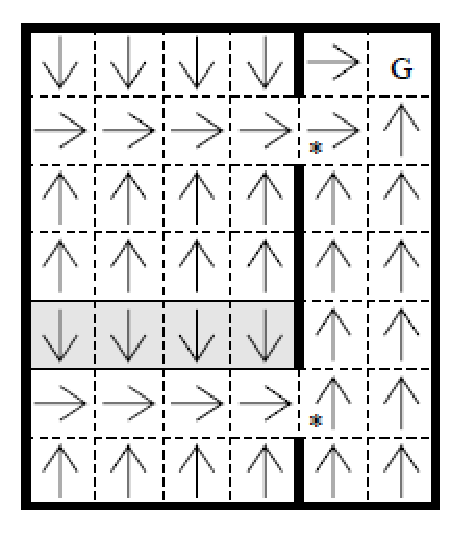
\includegraphics[width=2in] {./figures/Maze.eps}
\end{center}
\caption{A simple maze problem \cite{MaxQJ}.}
\label{fig:Maze}
\end{figure}
\begin{figure}[t]
\begin{center}
    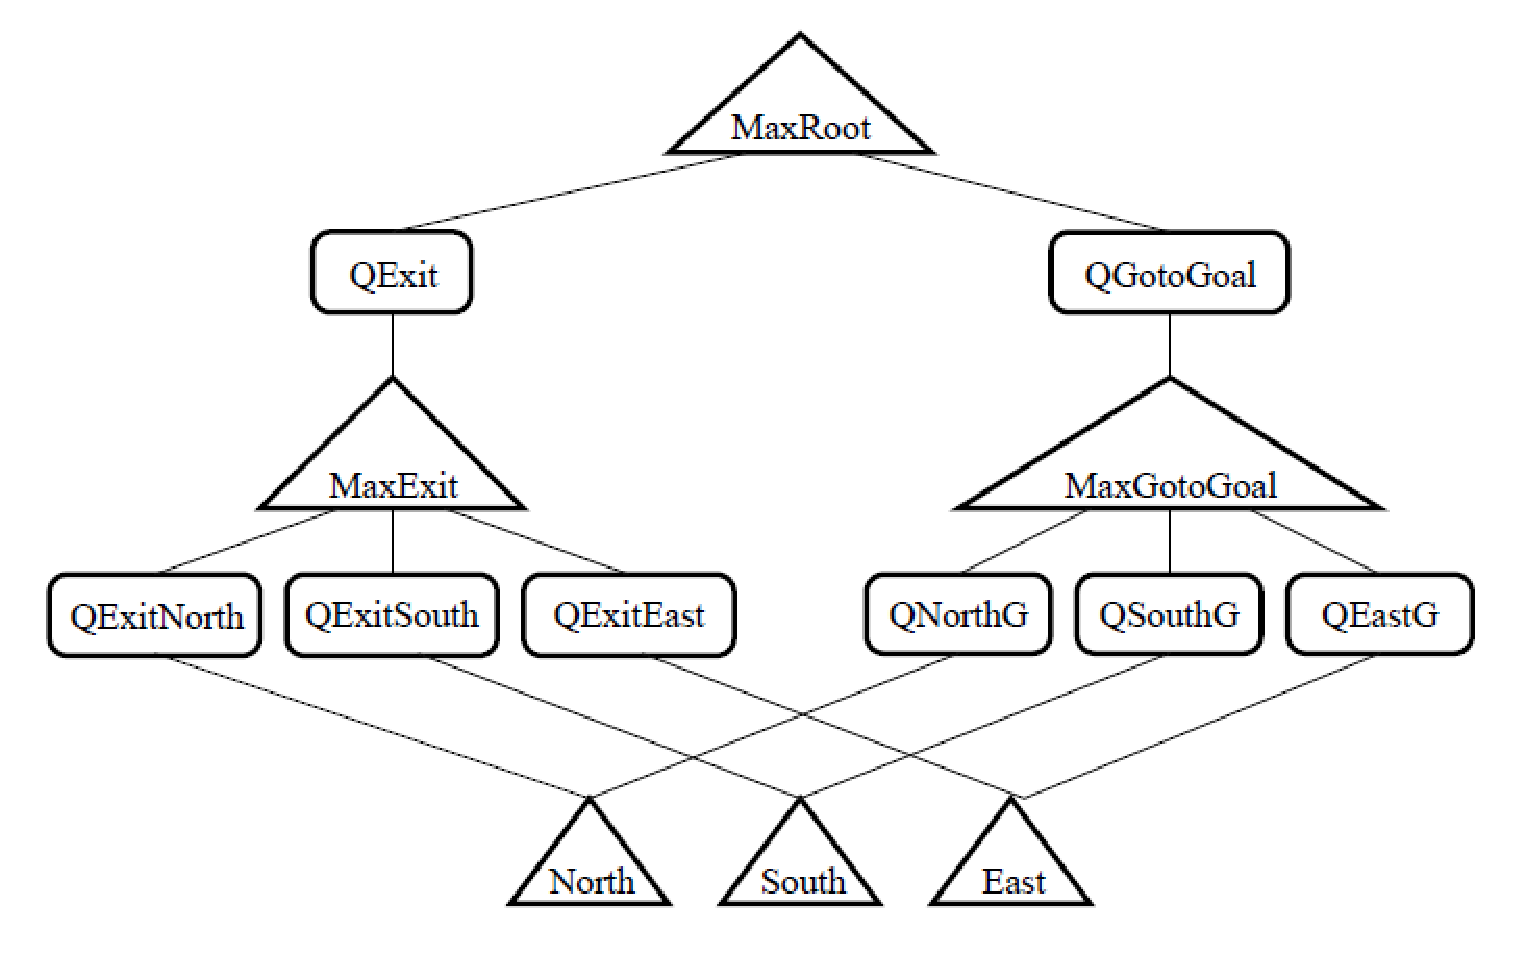
\includegraphics[width=4in] {./figures/MazeH.eps}
\end{center}
\caption{The task hierarchy of the simple maze problem.}
\label{fig:MazeH}
\end{figure}

There are three definitions of optimality in HRL:

\begin{definition}
    \textbf{Optimality:} An optimal policy $\pi^*$ for MDP $M$ is a policy that achieves the highest cumulative reward
    among all policies for the MDP.
\end{definition}
\begin{definition}
    \textbf{Recursive Optimality:} A recursively optimal policy for MDP $M$ with hierarchical 
    decomposition $M' = \{M_0, M_1, \dots, M_n\}$ is a policy $\pi = \{\pi_0, \pi_1, \dots, \pi_n\}$ such
    that each policy $\pi_i$ achieves the highest cumulative pseudo-reward for the corresponding subtask $M_i$,
    assuming fixed policies for its child subtasks.
\end{definition}
\begin{definition}
    \textbf{Hierarchical Optimality:} Given $Pi_H$, which is the set of all policies consistent with hierarchy $H$, 
    then a hierarchically optimal policy for MDP $M$ is a policy $\pi^* \in Pi_H$ that achieves the highest cumulative reward
    among all policies $\pi \in Pi_H$.
\end{definition}

An optimal policy is what we want to find for any MDP $M$. However, it may not be possible
due to the constraints imposed by the hierarchy. Instead of seeking optimality, 
we can seek hierarchical optimality or recursive optimality, which are two important 
optimality guarantees in HRL.

Recursive optimality guarantees that the policy of each subtask is optimal given the policies of its child subtasks.
In this form of optimality, each subtask learns the optimal policy while ignoring the policy from its ancestors
and the all subsequent rewards after the agent arrives the terminal states of the subtask.
Recursive optimality allows the policy of subtask to be reused for different hierarchies. Since
each subtask only needs to seek the optimality within its own subproblem, it is also possible
to adopt state abstraction by ignoring the state variables which are irrelevant
to the subproblem. The MAXQ-Q \cite{MaxQJ} algorithm converges to a recursively optimal policy. 

A hierarchically optimal policy is the policy which achieves the highest cumulative reward given the
hierarchical constraints. The hierarchically optimal policy is a stronger form of optimality. It
may achieve a higher cumulative reward than a recursively optimal policy. In hierarchical optimality, 
the policy of each subtask may not be optimal within its own subproblem, but the overall policy 
of the entire hierarchy is optimal. The HAMQ \cite{HAMQ}, SDMP \cite{SMDP}, tracked Q and HORDQ \cite{HORDQ} algorithms learn
a hierarchically optimal policy.

%TODO: pros and cons for HO and RO
Dietterich \cite{MaxQJ} demonstrates the difference of recursively and hierarchically optimal policies 
with a simple Maze problem (Figure \ref{fig:Maze}). A robot starts at left room and it needs to reach 
the goal $G$ in the right room. It has three primitive actions, North, South and East.  
The robot receives a reward of -1 for each move.
There are two subtasks, Exit and GotoGoal. Subtask Exit terminates when the robot exits the left room,
and GotoGoal terminates when the robot reaches the goal. The arrows in Figure \ref{fig:Maze} show the 
recursively optimal policy. The arrows in the left room indicate a policy which seeks to exit
the left room with minimum steps. The arrows in the right room seek a shortest path to the goal.
Note that the policy in the shaded area is recursively optimal but not hierarchically optimal nor
optimal. A hierarchically optimal policy should exit the left room by the upper door, but a recursively 
optimal policy always exits the room with minimum moves since
a recursively optimal policy ignores the consequences after the subgoal is achieved. 

%TODO: why do we need HO to do the optimal planning
Despite the fact that a hierarchically optimal policy is better than a recursively optimal policy, 
the algorithms which learn the hierarchically optimal policy do not always yield a speedup over
the flat algorithms such as Q-learning or SARSA \cite{MaxQJ, Andre02}. 


%\section{Pseudo-reward}


%%explain the reward system here
%%the difference between MAXQ's pseudo reward
%%explain my rewarding system here, and only add reward at terminal state
%One of the problem of hierarchical optimal learning algorithms is that policy $\pi_i$ of subtask $M_i$
%is determined by the reward of original MDP. There are no pseudo-rewards which are allowed as
%in MAXQ. Due to the lack of pseudo reward, each subtask $M_i$ lacks the motivation to 
%pursue the subgoal defined by the hierarchy, thus it makes the hierarchical 
%design useless. It is necessary to add some pseudo-rewards to encourage each subtask to pursue 
%the subgoal. However, we cannot guarantee optimality with a nonzero pseudo-reward.
%%use taxi domain to explain or maze problem (Navigate(t) problem)
%%a key is policy reuse

%%TODO: mention that pseudo-reward can atlernative between different policy
%In fact, the above argument illustrates the difference between the hierarchically optimal policy
%and the recursively optimal policy. 
%As shown in the expriment of \cite{Andre02}, hierarchically optimal RL learns  
%a better policy than the one of recursively optimal RL. However, its learning rate
%is slower than resursively optimal one.

%Since neither approach is better than the other in terms of learning rate and 
%the quality of policy, there are no reason to stick to one of them.
%With the introduction of pseudo-reward, we can alternate the agent's behavior
%between the hierarchically optimal RL and the recursively optimal RL.

%We show two tricks we can play when working with these pseudo-rewards.
%We showed that with the appropriately choosen pseudo-reward, the resulting behavior
%can be better than both approaches in terms of learning rate and the quality of policy.
%The result is presented in chapter 4.

%%a bridge between RO and HO

%A practical approach is to use positive reward to encourage the effective exploration
%in the early stage, and gradually decrease it to 0. 

%The penalty term serves as a mechanism to enforce the subtask to follow the hierarchy.
%The subtask will strictly follow the subgoal defined by the hierarchy if the penalty term is large.
%On the other hand, if the penalty term is small, the subtask is more likely to go rouge and try to 
%solve the whole problem on its own. Here we have a engineering decision: if we trust our hierarchy design, 
%we should increase the penalty term to let the agent find the optimal policy as fast as it can; 
%if not, a low penalty term allows the agent to find the optimal policy when the hierarchy doesn't work.

%\subsection{Taxi Domain}
%%Logic of Adaptive Behavior ->Options, SMDP, MAXQ, HORDQ, HAMQ
%MAXQ. The MAXQ algorithm (Dietterich, 1998, 2000b,a) can be seen as an extension
%of the HSMQ algorithm. It relies on the theory of SMDPs but unlike e.g. the options
%framework, it does not rely on reducing the complete problem to a single SMDP. Instead a
%hierarchical task decomposition in behaviors is assumed to be given, and learning proceeds
%in a way similar to SMDP- or HSMQ-learning. MAXQ learns policies equivalent to HSMQ,
%but in addition, it uses a sophisticated value function decomposition to learn these more
%134
%3.8 ABSTRACTION TYPE V: Hierarchical and Temporal Abstraction
%efficiently. The value of a behavior in the context of its calling parent behavior can be
%decomposed into i) the reward expected while executing it and ii) the discounted reward
%of continuing to execute the parent task after it terminates. Let P be the parent behavior
%of B, then
%QP(s; B) = IP(s; B) + CP(P; s; B)
%where IP(s; B) is the expected total discounted reward that is received while executing
%behavior B from initial state s and CP(P; s; B) is the expected total reward of continuing to
%execute behavior P after B has terminated, discounted appropriately with respect to the
%time spent on executing behavior B.
%Pickup
%North East
%t/source
%Put
%Putdown
%South West
%Get
%t/destination
%Root
%Navigate(t)
%Figure 3.18: An example of hierarchical abstraction:
%the MAXQ task hierarchy (Dietterich,
%2000a). The hierarchy constrains the policy space
%in the taxi domain. The leaves of the tree contain
%basic actions in the domain (such as North) and
%the inner nodes represent behaviors that are constructed
%using actions and behaviors lower in the
%tree. Note that the Navigate behavior is reused
%for both getting to the passenger and delivering
%him, and also that it is parameterized using the
%target location.
%The IP(s; B) can be recursively decomposed
%into I and C following
%IP(s; B) = max
%a2AB
%QP(s; a)
%There are several advantages of this decomposition,
%specifically in learning recursively
%optimal Q-values. Both the I and C functions
%can be represented using different state
%space abstractions, allowing for sharing (and
%compactness) in the representation of the
%value function. See (Dietterich, 2000a) for
%more subtle details on this decomposition.
%HAMQ. Q-learning with hierarchies of abstract
%machines (HAMQ) (Parr and Russell,
%1998) learns hierarchically optimal policies,
%and uses devices resembling finite-state machines
%to implement behaviors. These machines
%include an internal state and this state
%determines the actions that are taken. Like
%the options framework, HAMs are based on
%the SMDP model, though the aim here is not
%to enlarge the action space with behaviors, but instead to simplify large MDPs by restricting
%the policy space. The core idea in HAM is that the policies for the original MDP are
%defined as programs which execute based on their own state as well as the state of the
%underlying MDP. There are several types of actions. There are primitive actions, actions
%that terminate the current behavior and return control to the calling behavior and actions
%that call other behaviors. Learning takes place only at choice points where a behavior
%must decide which of several internal transitions to make. These choice-points represent
%a trade-off between fully hard-coded policies and learned policies. All the finite state machines
%representing the behaviors are compiled into one machine where the learning takes
%place. Andre and Russell (2001) extended the framework to programmable HAMs, adding
%interrupts and the ability to pass parameters, among other things, and later extended the
%programming language to ALISP (Andre and Russell, 2002, see also Chapter 7).



%subtasks were only partially specified. The MAXQ model is one of the first methods to
%combine temporal abstraction with state abstraction. It provides a more comprehensive
%framework for hierarchical learning where instead of policies for subtasks, the learner is
%given pseudo-reward functions. Unlike options and HAMs, MAXQ does not rely directly
%on reducing the entire problem to a single SMDP. Instead, a hierarchy of SMDPs is created
%whose solutions can be learned simultaneously. The key feature of MAXQ is the decomposed
%representation of the value function. Dietterich views each subtask as a separate
%MDP, and thus represents the value of a state within that MDP as composed of the reward
%for taking an action at that state (which might be composed of many rewards along a trajectory
%through a subtask) and the expected reward for completing the subtask. To isolate
%the subtask from the calling context, Dietterich uses the notion of a pseudo-reward. At the
%terminal states of a subtask, the agent is rewarded according to the pseudo-reward, which
%is set a priori by the designer, and does not depend on what happens after leaving the current
%subtask. Each subtask can then be treated in isolation from the rest of the problem
%with the caveat that the solutions learned are only recursively optimal. Each action in the
%recursively optimal policy is optimal with respect to the subtask containing the action, all
%descendant subtasks, and the pseudo-reward chosen by the designer of the system. Another

%machines (HAMQ) (Parr and Russell,
%1998) learns hierarchically optimal policies,
%and uses devices resembling finite-state machines
%to implement behaviors. These machines
%include an internal state and this state
%determines the actions that are taken. Like
%the options framework, HAMs are based on
%the SMDP model, though the aim here is not
%to enlarge the action space with behaviors, but instead to simplify large MDPs by restricting
%the policy space. The core idea in HAM is that the policies for the original MDP are
%defined as programs which execute based on their own state as well as the state of the
%underlying MDP. There are several types of actions. There are primitive actions, actions
%that terminate the current behavior and return control to the calling behavior and actions
%that call other behaviors. Learning takes place only at choice points where a behavior
%must decide which of several internal transitions to make. These choice-points represent
%a trade-off between fully hard-coded policies and learned policies. All the finite state machines
%representing the behaviors are compiled into one machine where the learning takes
%place. Andre and Russell (2001) extended the framework to programmable HAMs, adding
%interrupts and the ability to pass parameters, among other things, and later extended the
%programming language to ALISP (Andre and Russell, 2002, see also Chapter 7).

%Parr [48, 49] developed an approach to hierarchically structuring MDP policies called Hierarchies of Abstract
%Machines or HAMs. Like the options formalism, HAMs exploit the theory of SMDPs, but the emphasis is
%on simplifying complex MDPs by restricting the class of realizable policies rather than expanding the action
%choices. In this respect, as pointed out by Parr [48], it has much in common with the multilayer approach for
%controlling large Markov chains described by Forestier and Varaiya [20] who considered a two-layer structure
%in which the lower level controls the plant via one of a set of pre-de¯ned regulators. The higher level, the
%supervisor, monitors the behavior of the plant and intervenes when its state enters a set of boundary states.
%Intervention takes the form of switching to a new low-level regulator. This is not unlike many hybrid control
%methods [8] except that the low-level process is formalized as a ¯nite MDP and the supervisor's task as a
%¯nite SMDP. The supervisor's decisions occur whenever the plant reaches a boundary state, which e®ectively
%\erases" the intervening states from the supervisor's decision problem, thereby reducing its complexity [20].
%In the options framework, each option corresponds to a low-level regulator, and when the option set does not
%contain the one-step options corresponding to all primitive actions, the same simpli¯cation results. HAMs
%extend this idea by allowing policies to be speci¯ed as hierarchies of stochastic ¯nite-state machines.
%The idea of the HAM approach is that policies of a core MDP are de¯ned as programs which execute
%based on their own states as well as the current states of the core MDP.


%In
%the options model (at least in its simplest form), Sutton et. al. studied how to learn policies
%given fully specified policies for executing subtasks. In the HAMs formulation, Parr
%showed how hierarchical learning could be achieved even when the policies for lower-level
%subtasks were only partially specified. The MAXQ model is one of the first methods to
%combine temporal abstraction with state abstraction. It provides a more comprehensive
%framework for hierarchical learning where instead of policies for subtasks, the learner is
%given pseudo-reward functions. Unlike options and HAMs, MAXQ does not rely directly
%on reducing the entire problem to a single SMDP. Instead, a hierarchy of SMDPs is created
%whose solutions can be learned simultaneously. The key feature of MAXQ is the decomposed
%representation of the value function. Dietterich views each subtask as a separate
%MDP, and thus represents the value of a state within that MDP as composed of the reward
%for taking an action at that state (which might be composed of many rewards along a trajectory
%through a subtask) and the expected reward for completing the subtask. To isolate
%the subtask from the calling context, Dietterich uses the notion of a pseudo-reward. At the
%terminal states of a subtask, the agent is rewarded according to the pseudo-reward, which
%is set a priori by the designer, and does not depend on what happens after leaving the current
%subtask. Each subtask can then be treated in isolation from the rest of the problem
%with the caveat that the solutions learned are only recursively optimal. Each action in the
%recursively optimal policy is optimal with respect to the subtask containing the action, all
%descendant subtasks, and the pseudo-reward chosen by the designer of the system. Another
%important contribution of Dietterich’s work is the idea that state abstraction can be done
%separately on the different components of the value function, which allows one to perform
%more abstraction. We investigate the MAXQ framework and its related concepts such as
%pseudo-reward, recursive optimality, value function decomposition, and state abstraction in
%more details in Chapter 3. In the PHAMs model, Andre and Russell extended HAMs and
%presented an agent design language for RL. Andre and Russell (2002) also addressed the
%issue of safe state abstraction in HRL. Their method yields state abstraction while maintaining
%hierarchical optimality.




%In this chapter, we introduce a general hierarchical reinforcement learning (HRL) framework
%for simultaneous learning of policies at multiple levels of hierarchy. Our treatment
%builds upon the existing approaches such as HAMs (Parr, 1998), options (Sutton et al.,
%1999; Precup, 2000), MAXQ (Dietterich, 2000), and PHAMs (Andre and Russell, 2002;
%Andre, 2003), especially the MAXQ value function decomposition. In our framework,
%we add three-part value function decomposition (Andre and Russell, 2002) to guarantee
%hierarchical optimality, and reward shaping (Ng et al., 1999) to reduce the burden of exploration,
%to the MAXQ method. Rather than redundantly explain MAXQ and then our
%hierarchical framework, we will present our model and note throughout this chapter where
%the key pieces were inspired by or are directly related to Dietterich’s MAXQ work. In the
%following chapters, we first extend this framework to the average reward model, then we
%generalize it to be applicable to problems with continuous state and/or action spaces, and
%finally broaden it to be appropriate for domains with multiple cooperative agents.

%The difficulty with using the above methods was that decisions in HRL are no longer
%made at synchronous time steps, as is traditionally assumed in RL. Instead, agent makes decision
%in epochs of variable length, such as when a distinguishing state is reached (e.g., an
%intersection in a robot navigation task), or a subtask is completed (e.g., the elevator arrives
%on the first floor). Fortunately, a well-known statistical model is available to treat variable
%length actions: the SMDP model described in Section 2.3. Here, state transition dynamics
%is specified not only by the state where an action was taken, but also by parameters
%specifying the length of time since the action was taken. Early work in RL on the SMDP
%model studied extensions of algorithms such as Q-learning to continuous-time (Bradtke and
%Duff, 1995; Mahadevan et al., 1997b). The early work on SMDP model was then expanded
%to include hierarchical task models over fully or partially specified lower level subtasks,
%which led to developing powerful HRL models such as hierarchies of abstract machines
%(HAMs) (Parr, 1998), options (Sutton et al., 1999; Precup, 2000), MAXQ (Dietterich,
%2000), and programmable HAMs (PHAMs) (Andre and Russell, 2001; Andre, 2003). In
%the options model (at least in its simplest form), Sutton et. al. studied how to learn policies
%given fully specified policies for executing subtasks. In the HAMs formulation, Parr

%showed how hierarchical learning could be achieved even when the policies for lower-level
%subtasks were only partially specified. The MAXQ model is one of the first methods to
%combine temporal abstraction with state abstraction. It provides a more comprehensive
%framework for hierarchical learning where instead of policies for subtasks, the learner is
%given pseudo-reward functions. Unlike options and HAMs, MAXQ does not rely directly
%on reducing the entire problem to a single SMDP. Instead, a hierarchy of SMDPs is created
%whose solutions can be learned simultaneously. The key feature of MAXQ is the decomposed
%representation of the value function. Dietterich views each subtask as a separate
%MDP, and thus represents the value of a state within that MDP as composed of the reward
%for taking an action at that state (which might be composed of many rewards along a trajectory
%through a subtask) and the expected reward for completing the subtask. To isolate
%the subtask from the calling context, Dietterich uses the notion of a pseudo-reward. At the
%terminal states of a subtask, the agent is rewarded according to the pseudo-reward, which
%is set a priori by the designer, and does not depend on what happens after leaving the current
%subtask. Each subtask can then be treated in isolation from the rest of the problem
%with the caveat that the solutions learned are only recursively optimal. Each action in the
%recursively optimal policy is optimal with respect to the subtask containing the action, all
%descendant subtasks, and the pseudo-reward chosen by the designer of the system. Another
%important contribution of Dietterich’s work is the idea that state abstraction can be done
%separately on the different components of the value function, which allows one to perform
%more abstraction. We investigate the MAXQ framework and its related concepts such as
%pseudo-reward, recursive optimality, value function decomposition, and state abstraction in
%more details in Chapter 3. In the PHAMs model, Andre and Russell extended HAMs and
%presented an agent design language for RL. Andre and Russell (2002) also addressed the
%issue of safe state abstraction in HRL. Their method yields state abstraction while maintaining
%hierarchical optimality.

%It allows 
%assumes an MDP problem can be decomposed 
%into several smaller subtasks and 
%subtask. 
%Temporal abstraction is an important technique which has been studied extensively in
%clasicial AI and RL fields. The idea of hierarchical reinforckment learning (HRL) 
%is to decompose one monolith task into several smaller subtasks. Each subtask is 
%responsible to learn a policy of part of original state space. It allows reuse 
%the policy for 
%Reasoning and learning about temporally extended actions has been studied extensively
%in several fields including classical AI, control theory, and RL. In this section, we look at
%the historical development of hierarchy and temporal abstraction in classical AI, control,
%and RL
%Work in HRL has followed three main trends: focusing on
%subsets of the state space in a divide-and conquer approach (state space decomposition),
%34
%grouping sequences or sets of actions together (temporal abstraction), and ignoring differences
%between states based on the context (state abstraction). Much of the work falls into
%several of these categories.


%In this work, we follow the same hierarchical formulation as in MAXQ \cite{MaxQJ}:

%The following example from (Dietterich, 2000) demon-
%strates the dierence between recursively and hierar-
%chically optimal policies. Consider the simple maze
%problem in gure 1. Suppose a robot starts somewhere
%in the left room and it must reach the goal G in the
%right room. In addition to three primitive actions,
%North, South and East, the robot has a high level task
%Exit Room in the left room and a high level task Go to
%Goal in the right room. Exit Room terminates when
%the robot exits the left room and Go to Goal termi-
%nates when the robot reaches the goal G. The arrows
%in gure 1(a) show the locally optimal policy within
%each room. The arrows in the left room seek to exit
%the room by the shortest path. The arrows in the right
%room follow the shortest path to the goal. However,
%the resulting policy is not hierarchically optimal. Fig-
%ure 1(b) shows the hierarchically optimal policy that
%would always exit the left room by the upper door.
%This policy would not be locally optimal because the
%states in the shaded region would not follow the short-
%est path to the doorway.

%Recursive and hierarchical optimality are two impor-
%tant forms of optimality in hierarchical reinforcement
%learning. Recursive optimality only guarantees that
%the policy of each subtask is optimal given the policies
%of its children. It is an important form of optimality
%because it permits each subtask to learn a locally opti-
%mal policy while ignoring the behavior of its ancestors
%in the hierarchy. This increases the opportunities for
%subtask sharing and state abstraction. The original
%MAXQ HRL algorithm (Dietterich, 2000) converges
%to a recursively optimal policy. On the other hand,
%hierarchical optimality is a stronger form of optimal-
%ity since it is a global optimum consistent with the
%given hierarchy. In this form of optimality, the policy
%for each individual subtask is not necessarily optimal,
%but the policy for the entire hierarchy is optimal. The
%HAMQ HRL algorithm (Parr, 1998) and the SMDP
%learning algorithm for a xed set of options (Sutton
%et al., 1999) both converge to a hierarchically optimal
%policy.
%The following example from (Dietterich, 2000) demon-
%strates the dierence between recursively and hierar-
%chically optimal policies. Consider the simple maze
%problem in gure 1. Suppose a robot starts somewhere
%in the left room and it must reach the goal G in the
%right room. In addition to three primitive actions,
%North, South and East, the robot has a high level task
%Exit Room in the left room and a high level task Go to
%Goal in the right room. Exit Room terminates when
%the robot exits the left room and Go to Goal termi-
%nates when the robot reaches the goal G. The arrows
%in gure 1(a) show the locally optimal policy within
%each room. The arrows in the left room seek to exit
%the room by the shortest path. The arrows in the right
%room follow the shortest path to the goal. However,
%the resulting policy is not hierarchically optimal. Fig-
%ure 1(b) shows the hierarchically optimal policy that
%would always exit the left room by the upper door.
%This policy would not be locally optimal because the
%states in the shaded region would not follow the short-
%est path to the doorway.
